
\chapter{Tests et optimisations}
\label{chap:tests et optimisations}

\section{Premiers Tests de performance}

\subsection{Présentation}

Après avoir présenté les outils que nous avons utilisés, nous allons maintenant présenté les premiers tests de performances effectués avant la fin de l'optimisation.
Ces tests sont effectués à l'aide de la fonction time pour les temps d'exécution et valgrind pour les tests de mémoire.
Du fait de l'utilisation du langage C nous espérons avoir des temps bien inferieurs pour l'exécution de chaque programme, c'est ce que nous allons vérifier.
L'utilisation faite de la mémoire telle que le nombre d'allocations ou l'espace alloué par chaque programme ne dépend pas à priori du langage utilisé mais plutôt de l'algorithmie cachée dans le code, c'est pourquoi il ne devrait pas y avoir beacoup d'amèlioration de ce côté là,
néanmoins elle reste toujours un paramètre important faisant partie des performances d'un programme.
Nous avons ici classés les programmes comme dans la partie 2.

\subsection{Calculs simples sur des nombres d\'ecimaux}

Cette partie regroupe trois programmes : numaverage, numnormalize et numsum.
\newline

La fonction numsum n'étant pas encore fiinalisée cette section ne fera pas figuré de tests sur ce programme.
\newline

Ici le temps d'exécution varie selon le nombre de chiffre sur lequel on fait travailler un programme, c'est ce que nous allons observer.
La fonction numaverage comprend deux options principales. Elle permet de calculer à la fois, la moyenne, la médiane et le mode d'une série de nombre.
\newline

Voici un graphe en échelle logarithmique représentant le comportement des calculs de la médiane et de la moyenne en fonction du nombre de données. la fonction mode n'apparait pas car elle ne supporte pas bien les grands nombres de données et il n'y avait pas asser de points pour faire une courbe.
\newline

\begin{figure}
\begin{center}
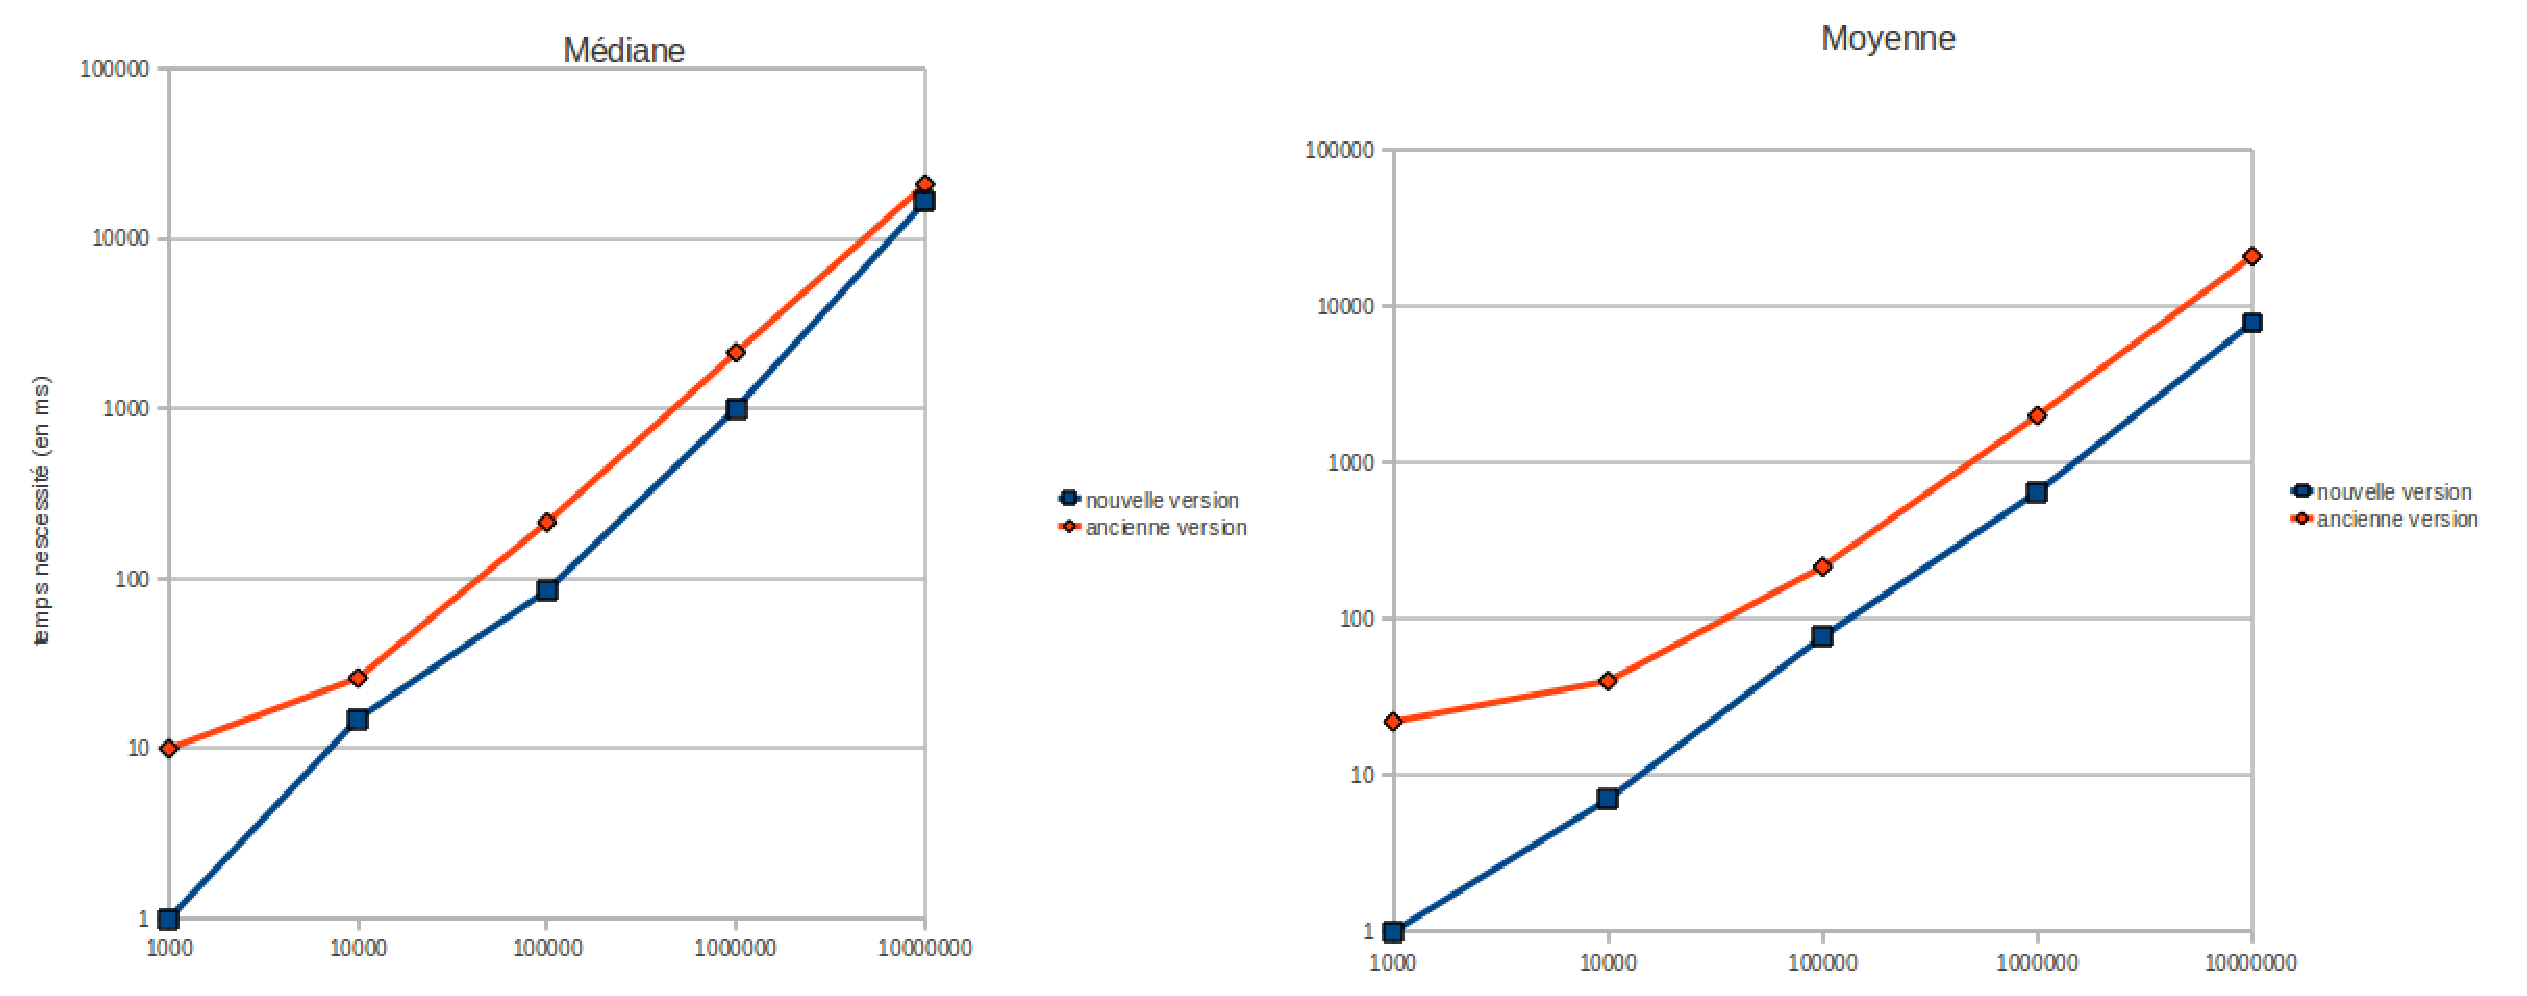
\includegraphics[width=15cm]{MoyenneMediane.eps}
\end{center}
\caption{Performances de Médiane et Moyenne}
\end{figure}

Et voilà un tableau relatant les performances de chacune de ces options (og et ng signifiant respectivement ``old version'' et ``new version'') : 
\newline


On voit successivement pour chaque test en première ligne le temps d'exécution en ms, en deuxième le nombre d'allocations et enfin en troisième la mémoire allouée.
\newline

\begin{tabular}{|c|c|c|c|c|c|c|}

\hline
Nb de données & moy (og) & moy (ng) & méd (og) & méd (ng) & mod (og) & mod (ng)  \\
\hline
 \multirow{3}*{1000} & 22 & 1 & 10 & 1 & 11 & 2 \\
\cline{2-7}
 & 1693 & 1 & 1693 & 1004 & 1693 & 2003 \\
\cline{2-7}
 & 183ko & 352o & 183ko & 4Mo & 183ko & 6Mo \\
\hline
 \multirow{3}*{10000} & 40 & 7 & 26 & 15 & 40 & 107 \\
\cline{2-7}
 & 1693 & 1 & 1693 & 10000 & 1693 & 2003 \\
\cline{2-7}
 & 183ko & 352o & 183ko & 400Mo & 183ko & 600Mo \\
\hline
100000 & 215 & 77 & 214 & 85 & 279 & 8024 \\
\hline
1000000 & 1991 & 647 & 2133 & 1004 &  &  \\
\hline
10000000 & 20748 & 7799 & 20802 & 16530 &  & \\
\hline

\end{tabular}

Remarque : Faute de temps (l'éxecution de valgrind étant très lente) les tests de mémoire n'ont pas été fait pour de grandes séries de nombre.

On peut remarquer que conformément à nos attentes les temps d'exécution des nouveaux programmes sont bien inferieurs à ceux des anciens, nénamoins certains d'entre-eux ont des consommations de mémoire beacoup plus importantes, cela est du au fait que certains de nos programme ne supportent pas encore les flux de données (en particulier la fonction qui calcule le mode), nous en reparlerons dans la partie optimisation.
Le problème de la gestion des flux de donnée est un problème récurrent en algorithmie : certains programmes ont besoins d'un historique des données pour faire leur calcul, ce qui devient un problème pour les grands nombres de données.

\subsection{Comparaisons de nombres d\'ecimaux}

Cette partie regroupe trois programmes : numbound, numinterval et numround.
\newline
Dans cette partie la problèmatique est quasiment la même que dans la partie précédente, à l'exception près qu'ici seulement la fonction numinterval est sujette au problème des flots de données.
\newline
On mettra ici le tableau et le graphique pour ces 3 fonctions.

\begin{tabular}{|c|c|c|c|c|}

\hline
Nb de données & numbound (og) & numbound (ng) & numround (og) & numround (ng) \\
\hline
1000 & 15 & 3 & 49 & 7 \\
\hline
10000 & 30 & 7 & 84 & 18 \\
\hline
100000 & 180 & 67 & 529 & 89 \\
\hline
1000000 & 2003 & 897 & 4152 & 1217 \\
\hline
10000000 & 19005 & 8669 & 42691 & 11842 \\
\hline

\end{tabular}
\newline

Les résultats sont particulièrement exceptionels en matière de temps d'exécution mais il persiste le problème de l'utilisation de la mémoire pour numinterval.



\subsection{G\'en\'eration et modifications de nombre d\'ecimaux}

Cette partie regroupe trois programmes : numgrep, numprocess, numrandom et numrange.
\newline

Dans cette partie la problèmatique est differente car aucun de ces programmes n'est destiné à travailler sur des flux de donnés, d'ailleur numrange et numrandom n'ont même pas de fichier en argument ils ne servent quèà génrer des nombres ou séries de nombres.


On peut ajouter que les programmes de l'ancienne bibliothèque comportent tous des fuites de mémoires (memory leaks) qui ne sont plus présent dans notre bibliothèque.

\section{Optimisation}